\chapter{I\lowercase{ntroduction}}

\section{Motivation}
Many real world applications use a feedback control policy to determine appropriate actions to apply to a dynamical system in order to achieve a given task. This policy makes its decision based on a set of measurements from the system. The procedure for designing such a policy is usually based on a mathematical model of the system in which simplifying assumptions may have been employed in the derivation. In many cases the equations of motion governing the system are unknown, or partially unknown, and building up a model based on physical intuition may be difficult. Therefore the question of how to design a control policy based on a combination of data obtained directly from interaction with the system and physical insight is an important one.


There are many techniques available to tackle problems of this kind based on different assumptions and levels of generality. There are also many issues that must be addressed. Do we adopt a model-based or model-free scheme? If a model-based scheme is used, what structure do we place on the dynamics of the system a priori? How do we deal with modelling uncertainty? How do we incorporate useful prior information about the system that we do know? In this thesis we define a probabilistic learning framework which addresses each of these issues, but with particular focus given to the latter. In particular, what are the advantages and potential pitfalls of forcing our prior beliefs into the learning framework.


\section{The Learning Framework}

The general framework we consider in this thesis is shown in \Fig{learnframe}. The system dynamics (which we consider to be in discrete-time) are governed by the function $\bff$ which we consider to be initially unknown or partially unknown. The goal is then to find a control policy $\bpi$, with free parameters $\bpsi$, to achieve a task. This task may be encoded in the scalar stage-cost $c$. System states are given by $\bx$ while actions are given by $\bu$. It is important to be clear at this stage that we have restricted our attention to scenarios in which we have access to measurements which completely determine the current state of a system. Therefore we do not explicitly deal with the problem of state estimation.



\begin{figure}[]
\centering
\subfigure[Model-free learning]{\tikzstyle{line} = [draw, -latex]
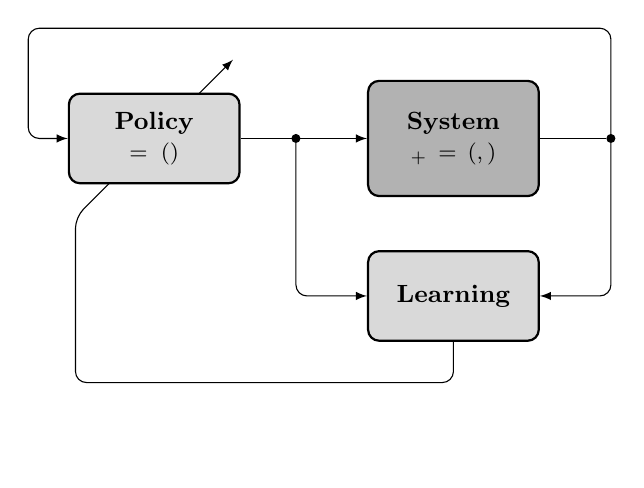
\begin{tikzpicture}[rounded corners, text centered]
\tikzstyle{dot} = [circle, draw, fill=black, inner sep=1pt]
  \small
  \node[draw, fill=white, white, thick, text width=6em, minimum height=3.5em] at (0,-3.5) {};
  \node[draw, thick, fill=black!15, text width=6em, minimum height=3.5em] at (0,-2) (learn){\bf Learning};
  \path[line] (learn.south) -- (0,-3.1) -| (-4.8,-1.0) -- (-2.8,1.0);

  \node[draw, thick, fill=black!15, text width=6em, minimum height=3.5em] at (-3.8,0) (pol){\bf Policy  \\ {\footnotesize $\bu = \bpi(\bx)$}};
  \node[draw, thick, fill=black!30, text width=6em, minimum height=4.5em] at (0,0) (sys){\bf System \\ {\footnotesize $\bx_+ = \bff(\bx,\bu)$}};

  
  \node[dot] at (-2,0) (dot1){};
  \node[dot] at (2,0) (dot2){};

  \path[draw] (sys.east) -- (dot2);
  \path[line] (dot1) |- (learn.west);
  \path[line] (dot2) |- (learn.east);
  \path[line] (dot2) |- (-5.4,1.4) |- (pol.west);
  \path[line] (pol.east) -- (sys.west);

  \node at (1.6,0.2) {$\bx$};
  \node at (-2,0.2) {$\bu$};
  \node at (-4.4,-2.8) {$\bpsi$};

\end{tikzpicture}
 \label{fig:learnframe}}
\subfigure[Model-based learning]{\tikzstyle{line} = [draw, -latex]
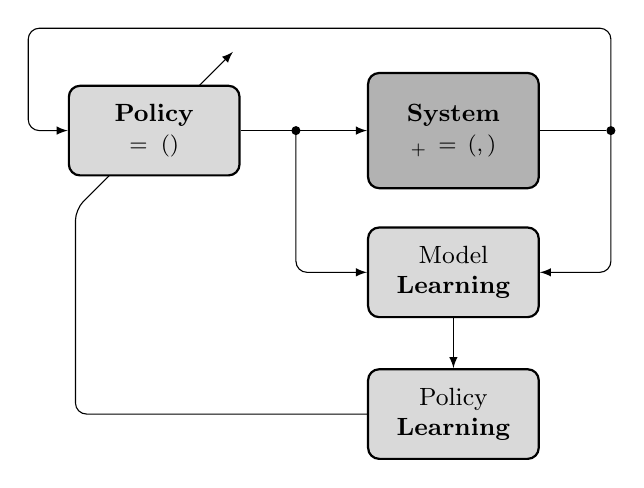
\begin{tikzpicture}[rounded corners, text centered]
\tikzstyle{dot} = [circle, draw, fill=black, inner sep=1pt]
  \small
  \node[draw, fill=black!15, thick, text width=6em, minimum height=3.5em] at (0,-3.6) (pilco){Policy \bf Learning};
  \path[line] (pilco.west) -| (-4.8,-1.0) -- (-2.8,1.0);

  \node[draw, thick, fill=black!15, text width=6em, minimum height=3.5em] at (-3.8,0) (pol){\bf Policy  \\ {\footnotesize $\bu = \bpi(\bx)$}};
  \node[draw, thick, fill=black!30, text width=6em, minimum height=4.5em] at (0,0) (sys){\bf System \\ {\footnotesize $\bx_+ = \bff(\bx,\bu)$}};
  \node[draw, thick, fill=black!15, text width=6em, minimum height=3.5em] at (0,-1.8) (GP){Model \bf Learning};
  
  \node[dot] at (-2,0) (dot1){};
  \node[dot] at (2,0) (dot2){};

  \path[draw] (sys.east) -- (dot2);
  \path[line] (dot2) |- (-5.4,1.3) |- (pol.west);
  \path[line] (pol.east) -- (sys.west);
  \path[line] (dot1) |- (GP.west);
  \path[line] (dot2) |- (GP.east);
  \path[line] (GP.south) -- (pilco.north);

  \node at (1.6,0.2) {$\bx$};
  \node at (-2,0.2) {$\bu$};
  %\node at (0.6,-2.85) {$\EE[\bw]$};
  \node at (-4.4,-3.35) {$\bpsi$};

\end{tikzpicture}
 \label{fig:learnframe2}}
\caption{These figures demonstrate the high level distinction between a model-free and model-based framework for learning control. Both frameworks are used for learning a parameterised discrete-time state-feedback control policy $\bpi$, mapping the system state $\bx$ to the control action $\bu$, to achieve some task or meet some performance criteria. The system has dynamics governed by the unknown function $\bff$ which maps the current state and action to the state at the following timestep $\bx_+$.}
\end{figure}


We consider now the distinction between \textit{model-free} and \textit{model-based} methods. The view we adopt for this thesis is that in a model-based method we can split the learning block into two parts: model learning and policy learning, as depicted in \Fig{learnframe2}. The model provides some kind of representation of the unknown system dynamics function $\bff$ which the learning block then makes use of when choosing the policy parameters. The learned model has the important property that it is able to generalise the information it has gained through interaction with the system based on some prior belief about the system dynamics. An example of such prior belief is the notion that states and actions that are close to each other, in some sense, will elicit similar responses from the system. We then take the view that a model free method adopts no such representation of the system dynamics during the design process.



What goes on in this learning process is the subject of much research. The two major fields which address the problem of designing algorithms for the learning block (and modelling block) are adaptive control and reinforcement learning, subfields of control theory and machine learning respectively. Although each field has very different roots, in recent years there has been much overlap in the problems they address. So before outlining our own solution to the control of initially unknown, or partially unknown, systems we shall consider a number of methods from the wide body of available literature across these two fields.











\chapter{R\lowercase{eview of the} L\lowercase{iterature}}


\section{Background}

Control theory is a discipline concerned with the behaviour of dynamical systems that can be specified by their inputs, states and outputs. The aim of control is to apply inputs to a system such that a desired output response is achieved. One of the standard assumptions in control theory is that a mathematical model of the system is available that describes its dynamic behaviour to a reasonable degree of accuracy. This model is then used as though it was the real system to design feedback control policies.

Among the most compelling arguments for the use of feedback rather than simply open loop control is that the effect of modelling uncertainty is reduced. Sometimes the discrepancy is so large however that the problem must be given further consideration. This is the subject of adaptive control. Adaptive control combines data obtained from interaction with the system with a control design procedure in order to adapt the policy online. The methods provided by the adaptive control community tend to place quite rigid assumptions on the form of the dynamics of the system.

Policy design for initially unknown systems has also been the subject of reinforcement learning. This is a framework born out of the Artificial Intelligence community and tackles the problem of learning a policy that is optimal with respect to some cost function given little or no prior knowledge about the system or environment. Originally these reinforcement learning methods were designed for systems with discrete state and input spaces, but recent advances have allowed algorithms for continuous systems to be defined.







\section{Adaptive Control}
\subsection{Introduction}
The methods in adaptive control can be split into \textit{direct} and \textit{indirect} algorithms. Direct adaptive control compares the system output response with some desired response and proceeds to adapt the controller parameters directly. Indirect adaptive control seeks to estimate unknown parameters in some system model and then uses this model to perform online controller design according to some design methodology. For a review of the fundamentals of the field, the reader is referred to the book by \cite{AsWi94} or the more recent text by \cite{IoFi06}.

As a side note, many reinforcement learning algorithms can in fact be viewed as direct adaptive control algorithms, as observed by \cite{SBW92}. While indirect methods are equivalent to model-based algorithms, since it means that an internal model of the system is maintained and used for policy design.
We shall now proceed to give an overview of a selection of the methods available in the literature for control of initially unknown or partially unknown systems.


\subsection{Model Reference Adaptive Control}
\subsubsection{Traditional Approach}
Model Reference Adaptive Control (MRAC) is a mechanism for adjusting policy parameters based on the error between the output of the actual plant and some desired plant $\be = \bx - \bx_m$. \Fig{MRAC} shows the general layout of an MRAC scheme, which generally operates on continuous-time systems. The original approach to MRAC was the celebrated ``MIT rule" $\dot\bpsi = - \gamma \be \nabla_{\bpsi} \be$ where $\gamma$ is a scalar to control the parameter rate of change and $\nabla_{\bpsi} \be$ is the so-called sensitivity derivative which must be approximated in some manner. This is equivalent to a continuous-time policy-gradient algorithm which finds the minimum of the cost function $J = \frac{1}{2}\be\T\be$ (discussed later). The currently favoured methods are that of Lyapunov-based design and the backstepping design of \cite{KKK95}. 

%%
\begin{figure}
\centering
\tikzstyle{line} = [draw, -latex]
\begin{tikzpicture}[rounded corners, text centered]
\tikzstyle{dot} = [circle, draw, fill=black, inner sep=1pt]
  \small
  \node[draw, thick, fill=black!15, text width=6em, minimum height=4.5em] at (0,-2.0) (learn){\bf Learning \\
{\footnotesize $\bs_+ = \bff_m(\bs)$ \\ $\bpsi = \bg(\be,\bu)$}};
  \path[line] (learn.south) -- (0,-3.1) -| (-4.8,-1.0) -- (-2.8,1.0);

  \node[draw, thick, fill=black!15, text width=6em, minimum height=3.5em] at (-3.8,0) (pol){\bf Policy  \\ {\footnotesize $\bu = \bpi(\bx)$}};
  \node[draw, thick, fill=black!30, text width=6em, minimum height=4.5em] at (0,0) (sys){\bf System \\ {\footnotesize $\bx_+ = \bff(\bx,\bu)$}};

  
  \node[dot] at (-2,0) (dot1){};
  \node[dot] at (2,0) (dot2){};

  \path[draw] (sys.east) -- (dot2);
  \path[line] (dot1) |- (learn.west);
  \path[line] (dot2) |- (learn.east);
  \path[line] (dot2) |- (-5.6,1.4) |- (pol.west);
  \path[line] (pol.east) -- (sys.west);

  \node at (1.6,0.2) {$\bx$};
  \node at (-2,0.2) {$\bu$};
  \node at (-4.4,-2.8) {$\bpsi$};

\end{tikzpicture}

\caption{Layout of an MRAC scheme where $\bff_m$ describes the ideal closed loop system and $\be$ is the error between the actual $\bx$ and ideal response $\bs$. The adaptation function $\bg$ can be determined through a variety of methods including stability theory.}
\label{fig:MRAC}
\end{figure}
%%


As an example, the Lyapunov-based design for MRAC is based on stability theory and in particular, Lyapunov's Direct Method. It consists of the following steps
\begin{enumerate}[	(1)]
\item Define a parameterised policy
\item Derive the error equation as a function of policy parameters
\item Find a Lyapunov function from which a parameter updating law can be defined such that the error will go to zero
\end{enumerate}
Now apply this to the linear system $\dot\bx = \bA\bx + \bB\bu$. We want the system to respond according to the model $\dot\bx_m = \bA_m\bx_m + \bB_m\br$ using some policy $\bu = \bpi_1(\br) - \bpi_2(\bx)$ with free parameters $\bpsi$. The closed loop system responds according to $\dot\bx = \bA_c(\bpsi)\bx + \bB_c(\bpsi) \br$. Therefore the error equation $\be = \bx - \bx_m$ has time derivative $\dot\be = \bA_m \be + (\bA_c(\bpsi) - \bA_m)\bx + (\bB_c(\bpsi) - \bB_m)\br = \bA_m \be + \Psi(\bpsi - \bpsi_0)$ for some matrix $\Psi$ and under the strong assumption that there exists a $\bpsi_0$ such that $\bA_c(\bpsi_0) = \bA_m$ and $\bB_c(\bpsi_0) = \bB_m$. Now introduce the Lyapunov function $V = \frac{1}{2}(\gamma \be^\top \bP \be + (\bpsi - \bpsi_0)^\top(\bpsi - \bpsi_0))$ for some positive definite matrix $\bP$. The associated time derivative is $\dot V = \frac{1}{2}\gamma \be^\top \bQ \be + (\bpsi - \bpsi_0)^\top \big(\dot\bpsi + \gamma\Psi^\top \bP \be \big)$ where $\bQ$ is positive definite and satisfies $\bA_m^\top \bP + \bP \bA_m = -\bQ$ (such a matrix will always exist if $\bA_m$ is stable). Therefore, choosing the update law $\dot\bpsi = - \gamma \Psi^\top \bP \be$ leads to a negative semidefinite $\dot V$ and using Barbalat's lemma, exponential decay to zero can be proven.
%
In practise it is usually impossible to implement the actual update law because one is unlikely to have access to the matrix $\Psi$ and therefore will have to approximate it in some manner.


For MRAC schemes in general, a reasonable degree of expert knowledge regarding the form of the system dynamics must be available in order to define a good adaptive law for the policy parameters. 



\subsubsection{Iterative Feedback Tuning}

Iterative Feedback Tuning (IFT) is a method of tuning the parameters of a policy in order to minimise some cost functional without knowledge of the plant dynamics. It was the contribution of \cite{HGG94} to show that an unbiased estimate of the gradient of the cost function with respect to policy parameters can be computed from signals obtained from closed loop experiments with the current policy operating on the actual system. These ideas were further developed and presented in the cornerstone paper of \cite{HGGL98}. On the other hand, in MRAC the true closed loop plant is replaced by the reference model in the gradient computation step. The minimisation of the cost function is then achieved using a Gauss-Newton based gradient descent scheme.

For the tuning of a one-degree of freedom controller, each gradient step consists of two batch experiments. The first is simply the collection of data under normal operating conditions while the second involves feeding back the output of the first experiment as the reference input to be tracked. This method has gained some acceptance in industry for the tuning of PID controllers due to its simplicity. The basic theory can be found in the survey paper of \cite{Hja02}.





\subsection{Self-Tuning Regulators}
\subsubsection{Traditional Approach}
Self-Tuning Regulators (STRs) maintain parameter approximations for a model of the system dynamics (usually a linear transfer function). This model is then used as part of an online control design scheme, for example pole placement or LQG. In general STRs are indirect adaptive methods since system parameters are learned explicitly. This framework is shown in \Fig{STRfig} where $\bw$ are the free parameters in the model and $\cD$ is the observed data set. However if an algebraic mapping straight to the policy parameters can be learned then it can be implemented as a direct method and can in fact be viewed as a form of MRAC.




The system model that is traditionally assumed in the STR framework is a Single Input Single Output (SISO) AutoRegressive with eXogenous inputs (ARX) model. This is defined as
\begin{equation*}
y_k = \bph^\top_{k-1} \bw + e_k
\end{equation*}
where $y_k$ is the output, $e \sim \cN(0,\sigma_e^2)$ is white noise, $\bph_{k-1} = [y_{k-1:k-n}; u_{k-m:k-n}; \hat e_{k-1:k-n}]$ is a vector of lagged outputs, inputs and estimated noise signals and $\bw$ is the vector of unknown parameters. Since these equations are linear in the unknown parameters $\bw$, we can employ standard Kalman filtering techniques to maintain a Gaussian distribution over this vector space $\bw \sim \cN(\bm_\bw,\bS_\bw)$. The equations used in this case would be
\begin{align*}
\bm_{\bw, k} &= \bm_{\bw, k-1} + \bK_k \Big( y_k - \bph\T_{k-1} \bm_{\bw, k-1} \Big) \\
\bS_{\bw, k} &= \Big(\bI - \bK_k\bph^\top_{k-1}\Big)\bS_{\bw, k-1}
\end{align*}
where $\bK_k = \bS_{\bw, k-1}\bph^\top_{k-1}\big( \sigma_e^2\bI + \bph^\top_{k-1} \bS_{\bw, k-1} \bph_{k-1}\big)\inv$ and assuming that we are given  prior measurements $\bph_0$ and an initial distriubtion $\bw_0 \sim \cN(\bm_{\bw, 0},\bS_{\bw, 0})$. The noise terms in $\bph_{k-1}$ cannot be measured directly in general, therefore they are replaced with estimates based on the current model. 

It is important to note that although an estimate of the full distribution over $\bw$ is maintained, in general only the mean prediction is used. This is due to the \textit{certainty equivalence principle} which assumes that the optimal control law is only dependent on the mean prediction of the parameter estimate.  \cite{TB75} prove that this principle holds for any known linear system with additive noise of known but arbitrary statistics, a measured output that is a nonlinear function of the state and noise (also with known but arbitrary statistics) and a quadratic cost function of state and input. However, it does not hold in the general case. It is this issue that is tackled by the framework of dual control which is outlined in \Sec{DC}.




%%
\begin{figure}
\centering
\tikzstyle{line} = [draw, -latex]
\begin{tikzpicture}[rounded corners, text centered]
\tikzstyle{dot} = [circle, draw, fill=black, inner sep=1pt]
  \small
  \node[draw, fill=black!15, thick, text width=6em, minimum height=3.5em] at (0,-3.6) (pilco){Policy \bf Learning};
  \path[line] (pilco.west) -| (-4.8,-1.0) -- (-2.8,1.0);

  \node[draw, thick, fill=black!15, text width=6em, minimum height=3.5em] at (-3.8,0) (pol){\bf Policy  \\ {\footnotesize $\bu = \bpi(\bx)$}};
  \node[draw, thick, fill=black!30, text width=6em, minimum height=4.5em] at (0,0) (sys){\bf System \\ {\footnotesize $\bx_+ = \bff(\bx,\bu)$}};
  \node[draw, thick, fill=black!15, text width=6em, minimum height=3.5em] at (0,-1.8) (GP){\bf Model \\ {\footnotesize $p(\bw|\cD)$ }};
  
  \node[dot] at (-2,0) (dot1){};
  \node[dot] at (2,0) (dot2){};

  \path[draw] (sys.east) -- (dot2);
  \path[line] (dot2) |- (-5.6,1.3) |- (pol.west);
  \path[line] (pol.east) -- (sys.west);
  \path[line] (dot1) |- (GP.west);
  \path[line] (dot2) |- (GP.east);
  \path[line] (GP.south) -- (pilco.north);

  \node at (1.6,0.2) {$\bx$};
  \node at (-2,0.2) {$\bu$};
  %\node at (0.6,-2.85) {$\EE[\bw]$};
  \node at (-4.4,-3.35) {$\bpsi$};

\end{tikzpicture}

\caption{Layout of an \textit{indirect} self-tuning regulator for a system described by the equations $\bx_+ = \bff(\bx,\bu)$ parameterised by the unknown or time-varying parameters $\bw$. First an estimate of the unknown parameters is made $\EE[\bw]$, then the estimated system model is used under some control design scheme to determine policy parameters $\bpsi$.}
\label{fig:STRfig}
\end{figure}
%%

The traditional STR scheme is then to perform an online policy design following some standard methodology using the estimated model of the plant as though it was the real plant. \cite{AsWi94} use either pole-placement or LQG methods for design which recursively solve a Diophantine equation or Riccati equation respectively. This would be an \textit{indirect} STR. A \textit{direct} STR can be obtained by combining the plant parameter estimation stage and the controller design to a problem where the controller parameters can be estimated directly.


\subsubsection{Adaptive Model Predictive Control}
The framework is of course much broader than these traditional methods. We could in fact consider a Model Predictive Control (MPC) scheme, in which the internal model is obtained through online estimation, to come under this framework. MPC uses an internal model of a system to perform an online optimisation over some finite predictive horizon and the space of possible control actions in order to determine the optimal sequence of actions to apply. It then applies the first (or first few) actions in this sequence to the real system and repeats the procedure at the subsequent timestep. One of the advantages of this method is that constraints on states and inputs can be handled quite naturally. For an excellent introductory resource to this control framework the reader is referred to \cite{Mac02}. 






\subsubsection{Dual Control} \label{sec:DC}
One issue with the STR scheme, and many other adaptive control methods, is how to ensure that the input signal under feedback is rich enough to excite the system in order to obtain good parameter estimates. In other words, is the input ``persistently exciting"? The desire to handle this problem in an optimal manner led to the notion of dual control.

Dual control was first introduced in the seminal papers by \cite{Fel61} and presented a theoretical framework for the optimal control of unknown, nonlinear stochastic systems. A helpful introduction can be found in \cite{Wit00}. The name dual control was given due to the fact that the resulting optimal control law sought to simultaneously control the system to the desired setpoint while introducing random probing inputs in order to improve parameter estimates. It was shown that the resulting control law was a function of the full distribution over the estimated values of model parameters $p(\bw)$, not just the mean prediction $\EE[\bw]$. The information contained in this full distribution is termed the \textit{hyperstate}. As previously discussed, this is in contrast to the vast majority of indirect STR algorithms.


In general the optimal dual solution is intractable and heuristic methods are employed to give a policy \textit{dual characteristics}. A survey of some of these approximation methods can be found in \cite{Wit95} and \cite{Un00}. \cite{TB72} provide an early example of a dual control heuristic showing significant improvement over the associated certainty equivalent scheme. Another example is that of \cite{FK97}, where an extra term is added in the cost function of a minimum-variance controller to induce dual action. \cite{SCT08} use a value function approximation scheme to solve the Hamilton-Jacobi-Bellman (HJB) equation for the dual control problem for a nonlinear system in which only a subset of the state variables were measured. The system dynamics are augmented with the dynamics of a Kalman-Bucy filter to yield a fully observable system. Then the value function is approximated using available training data and the optimal policy can be derived analytically, which is possible only because the considered system is affine in the inputs and quadratic in the input cost.







\subsection{Extremum Seeking Control}
\subsubsection{Background}
In some situations, the general setup given in \Fig{learnframe} can be decomposed into the form given in \Fig{statES}. In this case, the entire closed loop system has been reduced to a SISO static map $g$ (a form of cost function which is a function of the policy parameter $\psi$ directly) with no dynamics. In general, extremum seeking is not restricted to this assumption and can handle both dynamic maps and Multiple Input Multiple Output (MIMO) systems, but it allows an intuitive understanding of the method to be obtained. The aim is to find the optimal policy parameter $\psi^*$ to yield the optimal function value $g^*$.
%
An illustrative example is an anti-lock braking system in which there is a mapping from the desired slip of the wheel to the amount of friction generated. This mapping has some maximum value (in between no slip at all and skidding) which would be beneficial to operate at if the objective was to stop the vehicle as fast as possible. However the position of this maximum varies with changes in road condition, whether it is wet, dry, icy etc. The control methodology employs the use of an excitation or ``dither'' signal to provide an implicit search for the extremum. A recent real world example by \cite{BNTM09} is of its application in bioprocesses. 

\cite{ArKr03} claim that extremum-seeking was the original method of adaptive control, appearing as far back as the 1920s, developed mainly in the USSR during the 1940s and was popular in the 1950s and 1960s long before the theoretical breakthroughs in the adaptive control of linear systems in the 1980s. This popularity died down for a while, partly due to the difficulty in implementing optimizing controllers, however developments in computing power have led to a renewed interest, including the semi-plenary lecture given by \cite{Nes09}. There are two main approaches to extremum-seeking. One is the adaptive control method which makes use of a certain excitation or dither signal (often a sinusoid) to generate the desired suboptimal behaviour required to search for the extremum point. The other way is to use nonlinear programming techniques for numerical optimisation using probing inputs to generate an online approximation of the objective function gradient. By way of example, the adaptive control approach for an unknown static map will now be considered.



\begin{figure}
\centering
% Define block styles
\tikzstyle{block} = [rectangle, draw, text width=3em, text centered, rounded corners, minimum height=3em]
\tikzstyle{block2} = [rectangle, draw, text width=3em, text centered, rounded corners, minimum height=2em]
\tikzstyle{sum} = [thick, circle, draw, minimum height=.4cm]
\tikzstyle{line} = [draw, -latex]
\tikzstyle{dot} = [circle, draw, fill=black, inner sep=1pt, thick]
\begin{tikzpicture}[rounded corners]
	\small
	\draw[thick, fill = black!15] (-4,-5.3) rectangle (4,-1.7);
	\draw[thick, fill = black!30] (-2.1,-1) rectangle (2.1,1.3);
	% Place nodes
	\node at (0,0)[block](plant){$g(\psi)$};
	%\node at (-2.5,0)[sblock](iplant){$F_i(s)$};
	%\node at (2.5,0)[sblock](oplant){$F_o(s)$};
	%\node at (5,0)[dot](bit1){};
	\node at (0.5,-4.5)[dot](bit2){};
	\node at (2.5,-3)[block](highpass){$\quad$ \\[-0.75cm]\begin{equation*}\frac{s}{s+h}\end{equation*}};
	\node at (0.5,-3)[sum](mult){}; \node at (0.5,-3) {$\times$};
	\node at (-1.5,-3)[block](int){$\quad$ \\[-0.75cm]\begin{equation*}\frac{k}{s}\end{equation*}};
	\node at (-3.5,-3)[sum](add){}; \node at (-3.2,-2.7) {$-$};
	\node at (-1.5,-4.5)[block2](aaa){$a$};

	% Draw edges
	\path[line] (plant.east) -- (5,0)  |- (highpass.east);
	\path[line] (highpass.west) -- (mult);
	\path[line] (mult) -- (int.east);
	\path[line] (int.west) -- (add);
	\path[line] (add.west)  -| (-5,0) -- (plant.west);
	%\path [line] (plant.east) -- (oplant.west);
	%\path [line] (iplant.east) -- (plant.west);
	
	\path[line] (aaa.west) -| (add.south);
	\path[line] (aaa.east) +(2.6,0) -- (aaa.east);
	\path[line] (bit2) -- (mult.south);
	
	%\path[line] ([xshift=-.4cm]plant.north) +(0,.7) -- ([xshift=-.4cm]plant.north);
	%\path[line] ([xshift=.4cm]plant.north) +(0,.7) -- ([xshift=.4cm]plant.north);
	
	% Labels
	\node at (0,-2.05){\bf Adaptation};
	\node at (0,0.85){\bf Closed-Loop System};
	%\node at (0.45,1.5){$\psi^*$};
	%\node at (-0.35,1.5){$g^*$};
	\node at (2.5,-4.45){$\sin\omega t$};
	\node at (-4.5,-2.7){$\psi$};
	\node at (4.5,-2.7){$y$};
	\node at (-2.6,-2.7){$\hat\psi$};
	\node at (-0.2,-2.7){$\xi$};

\end{tikzpicture}
\caption{Layout of the extremum-seeking scheme with a sinusoidal dither signal of frequency $\omega$ for an unknown static map $g(\psi)$ with optimal value $g^*$ and associated setpoint $\psi^*$.}
\label{fig:statES}
\end{figure}

\subsubsection{Illustrative Example}
We will now gain some intuition as to how the scheme given in \Fig{statES} actually works. This example is outlined in \cite{ArKr03}. Assuming that the mapping $g$ is smooth then when the input $\psi$ is close to $\psi^*$ a locally valid approximation would be given by the quadratic
\begin{equation}
\label{eqn:staticmap}
g(\psi) = g^* + \frac{g''}{2}(\psi - \psi^*)^2
\end{equation}
where $g'':= \dd^2 g/\dd\psi^2 >0$ (if $g''<0$ simply replace $k$ ($k>0$) in \Fig{statES} with $-k$), $g^*$ and $\psi^*$ are unknown constants. The value $g^*$ is a local optimum of the general map. It is the dither signal $a \sin \omega t$ fed into the plant that helps get a measure of gradient information as will be illustrated in the following simple analysis. First observe that $\hat\psi$ is the estimate of the unknown optimal input $\psi^*$ and define the estimation error $\tilde{\psi} = \psi^* - \hat\psi$. When substituted into \Eq{staticmap} the following is obtained
\begin{align*}
y &= g^* + \frac{g''}{2}(\tilde\psi - a \sin \omega t)^2\\
&= g^* + \frac{a^2g''}{4} + \frac{a^2g''}{2}\tilde\psi^2 - ag''\tilde\psi\sin\omega t - \frac{a^2g''}{4}\cos2\omega t
\end{align*}
using basic trigonometric identities. The washout (high pass) filter $s/(s+h)$, with `corner frequency' $h$, then serves to remove the constant terms. After this the signal is demodulated through multiplication with $\sin \omega t$ as follows
\begin{align}
\nonumber\xi &\approx \frac{a^2g''}{2}\tilde\psi^2\sin\omega t - ag''\tilde\psi\sin^2\omega t - \frac{a^2g''}{4}\cos2\omega t\sin\omega t\\
&\approx  -\frac{a^2g''}{2}\tilde\psi  \quad+\quad  
\underbrace{\frac{a^2g''}{2}\tilde\psi\cos2\omega t + \frac{a^2g''}{8}(\sin\omega t - \sin3\omega t)}_
{\text{attenuated by the integrator } k/s} 
\quad+\!\!\!\!\!\!
\underbrace{\frac{g''}{2}\tilde\psi^2\sin\omega t }_{\text{negligible for local analysis}}
\label{eqn:xi}
\end{align}
again using basic trigonometric identities. Due to Lyapunov's Indirect Method the quadratic term in $\tilde\psi$ can be neglected as only local analysis is of interest. Assuming that $\omega$ is a relatively high frequency, the sinusoidal terms in \Eq{xi} would be significantly attenuated by the integrator. This leaves the following simple relationship
\begin{equation*}
\hat\psi \approx -\frac{k}{s}\left( -\frac{ag''}{2}\tilde\psi \right)
\end{equation*}
Finally, since $\psi^*$ is constant then $\dot{\tilde\psi} = -\dot{\hat\psi}$ so
\begin{equation*}
\dot{\tilde\psi} \approx -\frac{kag''}{2}\tilde\psi
\end{equation*}
Now since $kg''>0$, this is a stable system and it can be concluded that $\tilde\psi \rightarrow 0$, in other words the estimate $\hat\psi$ will converge to the the actual extremum $\psi^*$.


Discrete-time extremum seeking control is exactly analogous to the continuous-time as shown in \Fig{statES}. We can apply the Tustin transform $s \leftarrow 2(z-1)/\Dt(z+1)$, where $\Dt$ is the sampling period, to translate the integrator and the high pass filter to discrete equivalents. However, the stability proofs are quite different (see \cite{CKAL02}).








\section{Reinforcement Learning} %%%%%%%%%%%%%%%%%%%%%%%%%%%%%%%%%%%%
\subsection{Introduction}
Reinforcement learning is a field that was born, in the form that can be seen today, during the early 1980s. It was formed by the combination of two main threads of independent research. One thread was research carried out in optimal control and solutions involving the use of dynamic programming based methods. Although this did not involve learning as such, the algorithms gradually reach the correct solution through successive approximations so were considered among the other reinforcement learning methods. The other was research in learning by trial and error which started in the psychology of animal learning and led to Monte-Carlo methods for learning. Concepts from each of these threads were then combined to form a what is known as reinforcement learning today, a cornerstone of which were the Temporal Difference (TD) methods. One of the most famous successes of early TD methods came in the development of a world-class computer backgammon player in \cite{Tes92,Tes95}. Good reviews of the early literature in the field of reinforcement learning and the basic concepts can be found in \cite{SuBa98}, \cite{KLM96} and \cite{BerTs96} for a more in depth analysis.


\subsection{Markov Decision Process Framework}
Reinforcement learning algorithms assume the framework of a Markov Decision Process (MDP). MDPs are discrete-time dynamical systems where the next state is dependent only on the current state $\bx_k \in \XX \subset \RR^n$ and action $\bu_k \in \UU \subset \RR^m$ and governed by the mapping $\bff: \XX\times\UU\rightarrow\XX$. This property is known as the Markov property. Further, define $\bz := [\bx;\bu]$ as the combined state-action vector. The system is in some initial state drawn from the distribution $\bx_0 \sim p(\bx_0)$ and at any state $\bx_k$ the agent will draw an action from the stochastic policy $\pi(\bu_k|\bx_k)$, again parameterised by $\bpsi$. Note that the policy in this framework is considered as giving a distribution over actions rather than a deterministic mapping. However, usually once the learning phase is complete, the mean of this stochastic policy could be returned as a deterministic control policy.

A trajectory through the state-action space of an MDP is denoted $\btau = \{\bx_{0:H},\bu_{0:H}\} \in \mathcal{T}$ where $H$ is the task horizon. The probability of a trajectory being generated by a given policy is $p(\btau|\pi) = \pi(\bu_0|\bx_0) p_0(\bx_0)\prod_{k=1}^H \pi(\bu_k|\bx_k)$ according to the deterministic unknown dynamics function $\bff$ (stochastic dynamics may also be considered). The cost $\rho(\btau)$ for a given trajectory $\btau$ is defined as
\begin{equation*}
\rho(\btau) = \sum^H_{k=0} a_kc(\bz_k)
\end{equation*}
where $a_k$ is some time dependent weighting factor. Common examples are the \textit{discounted return} $a_k=\gamma^k$ where $\gamma \in (0,1]$ and the \textit{average return} $a_k = 1/(H+1)$. The general goal of reinforcement learning is to find a policy such that the expected cost
\begin{align*}
J(\pi) &= \EE_{\btau} \big[\rho(\btau) | \pi \big] = \int_{\mathcal{T}} \rho(\btau) P(\btau|\pi) \dd \btau
\end{align*}
is minimised. The policy which yields the minimum expected cost is denoted $\pi^* := \arg\min_\pi J(\pi)$.

We note that significant research is devoted to \textit{minimum regret} reinforcement learning. The notion of regret is to penalise the cost incurred by the algorithm during learning as well as the cost incurred by the final policy. Jointly addressing both of these issues is beyond the scope of this thesis therefore such algorithms will not be pursued further.


%
Important concepts in reinforcement learning and optimal control are that of the value function $V^\pi(\bx,k)$ and action-value function $Q^\pi(\bz,k)$. The value function is the expected return if policy $\pi$ is followed from state $\bx_k$. Similarly, the action-value function gives the expected return of taking action $\bu_k$ in state $\bx_k$ then choosing actions according to the policy $\pi$ thereafter. In mathematical terms 
\begin{align*}
V^\pi(\bx,k) &= \EE_{\btau}\Bigg[ \sum^H_{i=k} a_ic(\bz_i) \bigg|\bx_k=\bx,\pi \Bigg] \\
Q^\pi(\bz,k) &= \EE_{\btau}\Bigg[ \sum^H_{i=k} a_ic(\bz_i) \bigg|\bz_k=\bz,\pi \Bigg]
\end{align*}
If we restrict our attention to problems with time-invariant dynamics then in the infinite horizon case $H\rightarrow\infty$, these functions become time-invariant so are denoted $V^\pi(\bx)$ and $Q^\pi(\bz)$ respectively. Note that the expected return can be written in terms of the value function by averaging over all possible start states $\bx_0$, $J(\pi) = \int_{\XX} V^\pi(\bx_0)p(\bx_0)\dd\bx_0$.
The optimal value function is given by
\begin{equation*}
V^*(\bx) = \min_{\pi} [V^\pi(\bx)],
\end{equation*}
where an optimal policy is the argument to the minimal solution $\pi^*(\bx) = \arg\min_{\pi} V^\pi(\bx)$. The action-value function and value function are linked through the relationship $V^\pi(\bx) = \EE_{\bu} [Q^\pi(\bz)|\bx,\pi]$. Similarly, the optimal action-value function is related to the optimal value function through the relationship $V^*(\bx) = \min_{\bu \in \UU} [Q^*(\bz)]$.




\subsection{Dynamic Programming}
The dynamic programming paradigm of \cite{Bell57} is the framework that most reinforcement learning algorithms use to find an optimal policy. In order to introduce the concepts we shall restrict our attention to the infinite horizon ($H \rightarrow \infty$), discounted return ($a_k=\gamma^k$) case. It can be observed that the value function satisfies the Bellman (fixed-point) equation
\begin{equation*}
V^\pi(\bx) =  \EE_{\bx_+,\bu} \Big[ c(\bz) + \gamma V^\pi(\bx_+) \big|\bx,\pi \Big]
\end{equation*}
where $\bx_+ = \bff(\bx,\bu)$. Note that the uncertainty in $\bx_+$ comes from the stochastic policy $\pi$. The optimal value function satisfies the Bellman \textit{optimality} equation (otherwise known as the discrete-time Hamilton-Jacobi-Bellman (HJB) equation)
\begin{equation*}
V^*(\bx) = \min_{\bu\in\UU} \EE_{\bx_+} \Big[c(\bz) + \gamma V^*(\bx_+) \big|\bz\Big].
\end{equation*}
Given these equations we can now define two important forward in time algorithms: Policy Iteration and Value Iteration. Each one iterates between \textit{evaluation} of the value function of a given policy and \textit{improvement} of the policy but making it ``greedy" with respect to the current value function. These procedures are described in Algorithms~\ref{algo:polit} and \ref{algo:valit}.


%%
%\begin{wrapfigure}{r}{0.5 \textwidth}
%\begin{figure}
%\begin{center}
%% Define block styles
\tikzstyle{block} = [thick, rectangle, draw, text width=3em, text centered, rounded corners, minimum height=3em, fill=black!30]
\tikzstyle{line} = [draw, -latex]
\tikzstyle{dot} = [circle, draw, inner sep=1pt, fill=black]
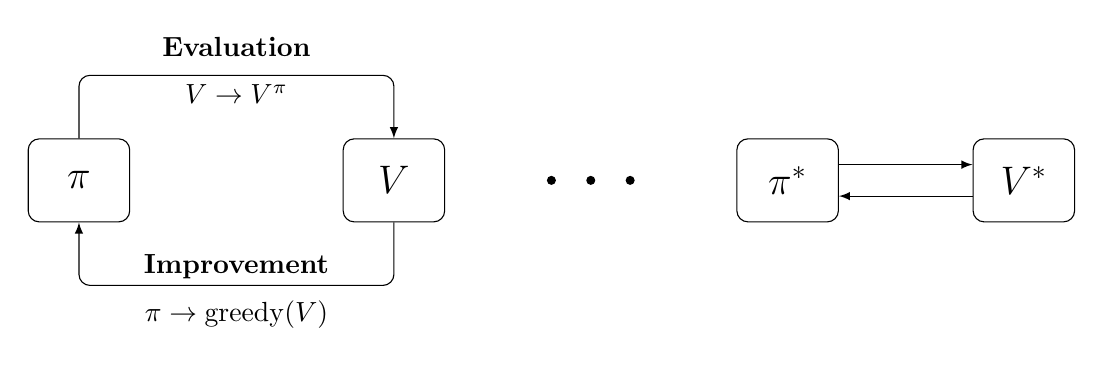
\begin{tikzpicture}[rounded corners]

	% Place nodes
	\node at(-2,0) [block](pie){\Large $\pi$};
	\node at(2,0) [block](vee){\Large $V$};
	\node at(7,0) [block](pie0){\Large $\pi^*$};
	\node at(10,0) [block](vee0){\Large $V^*$};
	
	\path[line] (pie.north) |- ([yshift=0.8cm]vee.north) -- (vee.north);
	\path[line] (vee.south) |- ([yshift=-0.8cm]pie.south) -- (pie.south);
	\path[line] ([yshift=0.2cm]pie0.east) -- ([yshift=0.2cm]vee0.west);
	\path[line] ([yshift=-0.2cm]vee0.west) -- ([yshift=-0.2cm]pie0.east);
	
	\node at (4,0)[dot]{}; \node at (4.5,0)[dot]{}; \node at (5,0)[dot]{};
	
	\node at (0,1.7){\textbf{Evaluation}};
	\node at (0,1.1){$V \rightarrow V^\pi$};
	\node at (0,-1.1){\textbf{Improvement}};
	\node at (0,-1.7){$\pi\rightarrow\mathrm{greedy}(V)$};

\end{tikzpicture}

%\end{center}
%\caption{Generalised Policy Iteration}
%\label{fig:GPI}
%\end{figure}
%\end{wrapfigure}
%%

\begin{algo}[Policy Iteration] \label{algo:polit}
Initialise procedure with some policy $\pi_0$. Iterate the following steps until convergence: 

\textbf{Evaluation:} Determine the value of policy $\pi_j$ by finding the value function $V_{j+1}$ that satisfies $V_{j+1}(\bx) = \EE_{\bx_+,\bu} \big[c(\bz) + \gamma V_{j+1}(\bx_+) |\bx,\pi_j \big]$.

\textbf{Improvement:} Determine an improved policy $\pi_{j+1}$ by being greedy with respect to the value function $V_{j+1}$ using $\pi_{j+1}(\bx) = \arg\min_{\bu\in\UU} \EE_{\bx_+} \big[ c(\bz) + \gamma V_{j+1}(\bx_+)|\bz\big]$.
\end{algo}

\begin{algo}[Value Iteration] \label{algo:valit}
Replace the evaluation step in Policy Iteration with a truncation by setting $V_{j+1}(\bx) = \EE_{\bx_+,\bu} \big[c(\bz) + \gamma V_{j}(\bx_+) |\bx,\pi_j\big]$ where $V_{j+1}$ has been replaced by $V_j$ on the right hand side.
\end{algo}

Both Policy Iteration and Value Iteration can be viewed under the Generalised Policy Iteration scheme of \cite{SuBa98} where evaluation and improvement steps are interleaved. In fact, all value function based schemes can be viewed under this framework.



Now, even if these algorithms were carried out using only data from interaction with the system, some a priori knowledge of the system dynamics is required in the improvement step, which is common to both algorithms. In order to find the minimal solution, the derivative with respect to the input $\bu$ is required which leads to the necessity of knowing the derivative $\partial\bff(\bx,\bu)/\partial\bu$ (the $``\bB"$ matrix if the system is linear). This problem is alleviated in reinforcement learning algorithms through the use of the action-value function in place of the value function. 
The action-value function satisfies
\begin{equation}
Q^\pi(\bz) = \EE_{\bz_+} \Big[ c(\bz) + \gamma Q^\pi(\bz_+) \big|\bz,\pi \Big]. \label{eqn:Qfixed}
\end{equation}
The optimal action-value function satisfies
\begin{equation*}
Q^*(\bz) = \EE_{\bx_+} \Big[ c(\bz) + \gamma \min_{\bu_+\in\UU}Q^*(\bz_+) \big|\bz \Big].
\end{equation*}
We shall now discuss how these can be used as the basis of practical algorithms.



\subsection{Temporal Differences}
\subsubsection{Bootstrapping Methods}
Bootstrapping methods are based on estimating the Temporal Difference (TD)-error which will be defined below. The term ``bootstrapping'' pertains to the idea that estimates of parameters are based on estimates of other parameters. These methods are ways of evaluating or estimating the value function of a given policy $V^\pi$ (not considered further, since knowledge of the system dynamics is required to find a policy), the action-value function $Q^\pi$ (the foundation of the $\SARSA$ algorithm) or the optimal action-value function $Q^*$ directly (the foundation of $\cQ$-learning). They have enjoyed much empirical success in the discrete state-space domain, including learning how to play backgammon \cite{Tes92,Tes95} and chess \cite{BTW00}. These methods utilise the TD-error, or Bellman error, as part of a stochastic gradient descent algorithm. In most applications it is necessary to maintain a parametric approximation of these functions, denoted by $\hat V_{\hyp}$ and $\hat Q_{\hyp}$ where $\hyp$ is the vector of free parameters. Borrowing from the survey paper of \cite{GP10b} the following cost functions are minimised
\begin{align}
J_{Q^{\pi}}(\hyp) &= \parallel Q^\pi - \hat Q_{\hyp} \parallel^2 \label{eqn:JQcost1} \\
J_{Q^*}(\hyp) &= \parallel Q^* - \hat Q_{\hyp} \parallel^2 \label{eqn:JQcost2}
\end{align}
for $\SARSA$ and $\cQ$-learning respectively. Finding the optimal setting for the parameters $\hyp$ is achieved using a stochastic gradient descent where the parameters are adjusted according to an approximation of the gradient of the cost function. Given an observation of a transition $(\bx,\bu,c,\bx_+,\bu_+)$ for $\SARSA$ or $(\bx,\bu,c,\bx_+)$ for $\mathcal{Q}$-learning the update law is given by
\begin{equation*}
\hyp_i = \hyp_{i-1} + \alpha_i \Big( \nabla_{\hyp_{i-1}}\hat Q_{\hyp}(\bz) \Big) \Delta_{i}
\end{equation*}
where $\alpha_i$ is a learning rate that satisfies the classical stochastic approximation criterion $\sum^\infty_{i=1} \alpha_i = \infty, \sum^\infty_{i=1} \alpha_i^2 < \infty$ and the TD-error $\Delta_{i}$ is given by
\begin{align*}
\Delta_{i} &=  \Big(c(\bz) + \gamma \hat Q_{\hyp_{i-1}}(\bz_+) \Big) - \hat Q_{\hyp_{i-1}}(\bz) \\
\Delta_{i} &=  \Big(c(\bz) + \gamma \min_{\bu_+ \in \UU}\hat Q_{\hyp_{i-1}}(\bz_+) \Big) - \hat Q_{\hyp_{i-1}}(\bz)
\end{align*}
for $\SARSA$ and $\cQ$-learning respectively. It should be noted that in approximating the action-value function (as in \SARSA) the agent must be following the policy $\pi$ in order to converge. This is known as an \textit{on-policy} method. A convergence proof of $\SARSA$ with linear function approximation in finite state-action space can be found in \cite{TV97}. $\cQ$-learning was introduced for the discrete space, look-up table formulation, in the thesis by \cite{Wat89} with convergence proofs following in \cite{WD92}. It is an \textit{off-policy} method since it can follow an arbitrary policy (provided it explores sufficiently in the state-action space) but will converge to the optimal action-value function. %The proof of convergence for both $\SARSA$ and $\cQ$-learning with linear function approximation, continuous state space and finite action space followed much later in \cite{MMR09}.


An important extension of the standard $\cQ$-learning algorithm: fitted $\cQ$-iteration, was presented by \cite{EGW05} and seeks to combine the $\cQ$-learning principle with supervised learning methods to form a batch algorithm.
A comparison of this approach with MPC can be found in \cite{EGCW09}.


\subsubsection{Residual Methods}
As opposed to minimising the cost functions given by (\ref{eqn:JQcost1}) and (\ref{eqn:JQcost2}) one could minimise the error obtained by forcing the function approximation $\hat Q_{\hyp}$ to satisfy the fixed point equation (\ref{eqn:Qfixed})
\begin{equation*}
J(\hyp) = \parallel \hat Q_{\hyp} - (c + \gamma \hat Q_{\hyp}) \parallel^2.
\end{equation*}
This method does not lend itself to the stochastic gradient descent method outlined in the previous section because a penalty term arises which acts to favour smooth functions and hence gives a biased estimate of the optimal solution. However, least squares approaches to this minimisation have worked well. For example Gaussian Process Temporal Differences (GPTD) of \cite{EMM03,EMM05} or Kalman Temporal Differences (KTD) of \cite{GPF09} (see \cite{GP10a} for a full derivation).



\subsubsection{Practical Issues}
There are a few notable problems with the algorithms outlined in this section. First, there is the problem of reconstructing a useable or parameterised policy from the action-value function once it has been learned (a notable exception is when the system is affine and the cost is quadratic in the control actions). However, the most important problem is that these methods do not scale to continuous state-action spaces. The reason for this is that the algorithms are not able to generalise what they have learned in one area of the state-action space to another, they have no notion that states that are ``close" to each other will respond in a similar way. Neglecting to include any such prior information means that all states must be visited individually in order to build a policy. This is impossible in continuous states.

% and problems of practical interest where it is unreasonable to search the entire state-action space (except the fitted Q-iteration algorithm). 

One class of reinforcement learning algorithms that has been able to overcome these issues is policy-gradient algorithms and are the subject of the following section.







\subsection{Policy-Gradient Algorithms}
\subsubsection{Background}
The aim of policy-gradient algorithms is to directly adjust policy parameters $\bpsi$ by utilising an estimate of the gradient of the expected return with respect to the policy parameters $\nabla  J(\bpsi)$. Note that $\nabla = \nabla_{\bpsi}$ unless otherwise specified. Such algorithms are often referred to as \textit{Actor-Critic Methods} where the \textit{critic} maintains the estimate of the action-value function which in turn informs the \textit{actor} how to update its parameters. The actor-critic layout is shown in \Fig{actorcritic}. Note that from an adaptive control perspective, this is a \textit{direct} method since it provides an update rule for the policy parameters directly. The policy parameters of the actor are updated in the direction of the negative gradient provided by the critic according to the adjustment law
\begin{equation*}
\bpsi_{i+1} = \bpsi_{i} - \alpha_i \nabla J(\bpsi)|_{\bpsi=\bpsi_i}
\end{equation*}
where the learning rate $\alpha_i$ satisfies $\sum_{i=0}^{\infty} a_i = \infty$ and $\sum_{i=0}^{\infty} a_i^2 < \infty$. Since the policy $\pi$ is now fully characterised by its free parameters $\bpsi$ the expected return $J(\pi)$ can be written $J(\bpsi)$.



The problem here is how do we obtain a good estimate of the gradient? Two prominent approaches can be found in the literature: finite-difference and likelihood ratio methods. For an overview of these methods the reader is directed to the article by \cite{PS08}. Finite-difference methods can be dated back as far as the 1950s, originating in the stochastic simulation community. They involve simply applying the policy to the system a number of times using slightly perturbed parameters $\bpsi+\Delta\bpsi$ each time. The gradient estimation problem is then turned into a regression problem. However, determining the size of $\Delta\bpsi$ requires good knowledge of the system and can be hard to tune without expert guidance. For this reason, these methods shall not be pursued further. Likelihood ratio methods are based on the \textit{likelihood ratio trick}.

%\cite{Mun06} provides an alternative to the likelihood ratio method that is not subject to variance explosion at the discrete timesteps approach zero. This is a neat theoretical trick but it does not come with a practically implementable algorithm.


%%
\begin{figure}
\centering
\tikzstyle{line} = [draw, -latex]
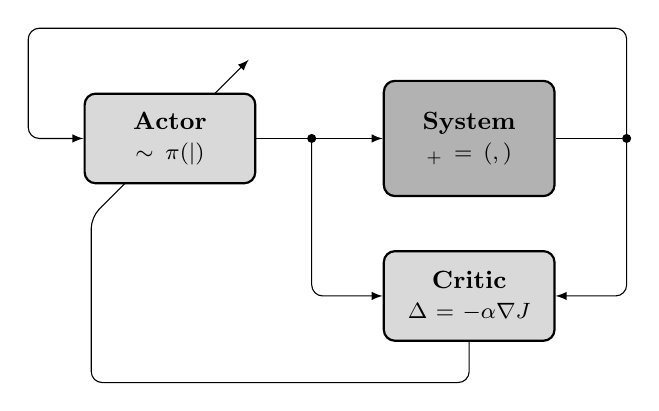
\begin{tikzpicture}[rounded corners, text centered]
\tikzstyle{dot} = [circle, draw, fill=black, inner sep=1pt]
  \small
  \node[draw, thick, fill=black!15, text width=6em, minimum height=3.5em] at (0,-2) (learn){\bf Critic \\ {\footnotesize $\Delta \bpsi = -\alpha \nabla J$}};
  \path[line] (learn.south) -- (0,-3.1) -| (-4.8,-1.0) -- (-2.8,1.0);

  \node[draw, thick, fill=black!15, text width=6em, minimum height=3.5em] at (-3.8,0) (pol){\bf Actor  \\ {\footnotesize $\bu \sim \pi(\bu|\bx)$}};
  \node[draw, thick, fill=black!30, text width=6em, minimum height=4.5em] at (0,0) (sys){\bf System \\ {\footnotesize $\bx_+ = \bff(\bx,\bu)$}};

  
  \node[dot] at (-2,0) (dot1){};
  \node[dot] at (2,0) (dot2){};

  \path[draw] (sys.east) -- (dot2);
  \path[line] (dot1) |- (learn.west);
  \path[line] (dot2) |- (learn.east);
  \path[line] (dot2) |- (-5.6,1.4) |- (pol.west);
  \path[line] (pol.east) -- (sys.west);

  \node at (1.6,0.2) {$\bx$};
  \node at (-2,0.2) {$\bu$};
  \node at (-4.4,-2.8) {$\bpsi$};

\end{tikzpicture}

\caption{Layout of the actor-critic policy gradient scheme where the policy is updated according to the rule $\bpsi \leftarrow \bpsi + \Delta\bpsi$. Note that the actor applies the policy and the critic updates the parameters.}
\label{fig:actorcritic}
\end{figure}
%%


\subsubsection{The Likelihood Ratio Trick}
The gradient of the expected return can be written analytically as
\begin{align*}
\nabla J(\bpsi) &= \int_{\cT} \rho(\btau) \nabla P(\btau|\pi) \dd \btau \\
&= \int_{\cT}  \rho(\btau) P(\btau|\pi)\nabla\log P(\btau|\pi) \dd \btau \\
&= \EE_{\btau} \Big[ \big(\rho(\btau) - b\big) \nabla\log P(\btau|\pi)  \big|\pi \Big].
\end{align*}
where the introduction of the arbitrary constant $b$ is possible since $\int_{\cT}b \nabla  P(\btau|\pi) \dd \btau = 0$, which is clearly true because $\int_{\cT}P(\btau|\pi) \dd \btau = 1$. This form is useful in two ways. The first is that it lends itself to sample based approximation given a set of trajectories sampled from the MDP using policy parameters $\bpsi$. Secondly, the term $\nabla \log P(\btau|\pi) = \sum_{k=0}^H \nabla \log \pi(\bu_k|\bx_k)$ requires no knowledge of the system dynamics to calculate. 
%
This is the basis of the episodic REINFORCE algorithm of \cite{Wil92}. Although $b$ has no effect on the mean of the gradient estimate it can have a huge effect on the variance of the estimate and can be chosen so as to minimise this variance. The optimal baseline was derived by \cite{PS08}. Improved algorithms were developed by \cite{SMSM00} and \cite{MT01} with the Policy Gradient Theorem and \cite{BB01} with GPOMDP. They make the intuitive observation that future actions are independent of past rewards. \cite{PS08} show from a trajectory based perspective that these algorithms are in fact equivalent. We shall now look further at the Policy Gradient Theorem.

\subsubsection{The Policy Gradient Theorem}
Consider the infinite horizon, normalised case, in which $\lim_{H\rightarrow\infty}\tfrac{1}{H}\sum_{k=0}^H a_k=1$. It was noted by \cite{SMSM00} that the expected return can be written in state-space form
\begin{equation*}
J(\bpsi) = \int_{\XX} d^\pi(\bx) \int_{\UU} \pi(\bu|\bx) c(\bx,\bu) \dd\bu\dd\bx
\end{equation*}
where $d^\pi(\bx) = \sum_{k=0}^\infty a_kp(\bx_k=\bx)$ is the weighted state distribution which is assumed to be independent of $\bx_0$ for all policies. Note that the control policy must be chosen carefully in order to make this a reasonable assumption. Setting the problem up in this way led to \Theo{polgrad}.

\begin{theo}[Policy Gradient Theorem]
For any MDP and arbitrary baseline $b^\pi(\bx)$ the following relationship holds 
\begin{equation*}
\nabla  J(\bpsi) = \int_{\XX} d^\pi(\bx) \int_{\UU} \nabla  \pi(\bx|\bu) \Big( Q^\pi(\bx,\bu) - b^\pi(\bx) \Big) \dd\bu\dd\bx
\end{equation*}
\label{theo:polgrad}
\end{theo}
\begin{proof}
The interested reader is directed to Theorem 1 in \cite{MT01} or Proposition 1 in \cite{SMSM00} for the original derivations.
\qed
\end{proof}

It was further shown by \cite{MT01} and \cite{SMSM00} that the term $Q^\pi(\bz) - b^\pi(\bx)$ can be replaced by a \textit{compatible function approximation} 
$f^\pi_{\hyp}(\bz) = \nabla  \log \pi(\bu|\bx)\T \hyp $
which does not affect the unbiasedness of the gradient estimate and is irrespective of the choice of baseline. Substituting this into the gradient equation from \Theo{polgrad} yields
\begin{equation*}
\nabla  J(\bpsi) = \int_{\XX} d^\pi(\bx) \mathbf{\hat G}_{\hyp}(\bx) \dd\bx \; \hyp = \mathbf{G}_{\hyp} \hyp
\end{equation*}
where the integral $\mathbf{\hat G}_{\hyp}(\bx) = \int_{\UU} \pi(\bu|\bx)\nabla \log\pi(\bu|\bx)\nabla \log\pi(\bu|\bx)^\top \dd\bu$ can be evaluated analytically since $\pi(\bu|\bx)$ is specified by the user. However, evaluating $\mathbf{G}_{\hyp}$ is still expensive since the stationary distribution $d^\pi(\bx)$ is unknown.

A major issue with the algorithms discussed so far is that they tend to reduce exploration noise in the policy too quickly and therefore converge slowly on the optimal solution. \cite{Kak02} showed that this problem is a product of using the standard gradient metric but can be overcome through the use of the \textit{natural policy gradient}.


\subsubsection{The Natural Policy Gradient}
Rather than following the steepest direction in parameter space the natural gradient follows the steepest descent direction with respect to the Fisher information matrix $\mathbf{F}_{\hyp}$
\begin{equation*}
\tilde\nabla  J(\bpsi) = \mathbf{F}_{\hyp}^{-1} \nabla  J(\bpsi)
\end{equation*}
The method came out of the supervised learning community where \cite{Ama98} showed that the natural gradient is superior to the standard gradient method since it exploits the properties of Riemannian manifolds. It was first utilised in a reinforcement learning context by \cite{Kak02} who demonstrated improved performance over the standard method. But it was the contribution of \cite{PVS05} to show that the Fisher information matrix $\mathbf{F}_{\hyp}$ is in fact identically equal to the matrix $\mathbf{G}_{\hyp}$ derived in the previous section. Therefore, utilising natural policy gradients we have the very elegant result that
\begin{equation*}
\tilde\nabla J(\bpsi) = \mathbf{F}_{\hyp}^{-1} \mathbf{G}_{\hyp} \hyp = \hyp
\end{equation*}
Therefore the only remaining issue is to estimate the parameter vector $\hyp$ of the compatible function approximation.
It is important and interesting to note that $f^\pi_{\hyp}(\bz)$ is mean zero with respect to the action distribution $\big(\int_{\UU} \pi(\bu|\bx) f^\pi_{\hyp}(\bz)\dd\bu = \hyp^\top \nabla\int_{\UU} \pi(\bu|\bx)\dd\bu =0 \big)$. Therefore it represents an \textit{advantage function} $A^\pi(\bz) = Q^\pi(\bz) - V^\pi(\bx)$ implying that the baseline $b^\pi(\bx)$ has implicitly been set to the value function. However, the advantage function cannot be estimated using TD-like bootstrapping methods without also maintaining an estimate of the value function $V^\pi(\bx)$ which can lead to problems if the function approximation scheme is chosen inappropriately.

This problem can be overcome with a couple of mild assumptions resulting in the Episodic Natural Actor-Critic algorithm of \cite{PVS05}. A Bellman-like equation in terms of the advantage function can be written as
\begin{equation*}
\sum_{k=0}^H a_k A^\pi(\bz_k) = a_{H+1}V^\pi(\bx_k) + \sum_{k=0}^H a_k c(\bz_k) - V^\pi(\bx_0)
\end{equation*}
Therefore, assuming a long task horizon $a_{H+1} \rightarrow 0$ (or $c(\bz_H)$ is the final cost) and a narrow start state distribution so that $V^\pi(\bx_0)$ can be approximated by a single scalar $J_0$, a simple regression problem results
\begin{equation*}
\sum_{k=0}^H a_k \nabla\log\pi(\bz_k)^\top \hyp + J_0 = \sum_{k=0}^H a_k c(\bz_k)
\end{equation*}
with $\mathrm{dim}\hyp +1$ unknowns. So for a deterministic system, only $\mathrm{dim}\hyp +1$ rollouts are required to find the natural gradient using least-squares regression
$[\hyp; J_0 ] = (\bPh^\top \bPh)^{-1} \bPh^\top\bPsi$
where $\Phi[i,:] = \big[\sum_{k=0}^H a_k \nabla\log\pi(\bu_{i,k}|\bx_{i,k})^\top,1\big]$ and $\Psi[i] = \sum_{k=0}^H a_kc(\bz_{i,k})$ with $\bz_{i,k}$ representing $\bz_k$ taken from the $i\tth$ rollout.




%%
%\begin{figure}
%\centering
%\tikzstyle{line} = [draw, -latex]
\begin{tikzpicture}[rounded corners, text centered]
\tikzstyle{dot} = [circle, draw, fill=black, inner sep=1pt]
  \small
  \node[draw, fill=black!15, thick, text width=6em, minimum height=3.5em] at (0,-3.5) (pilco){\bf Learning};
  \path[line] (pilco.west) -| (-4.8,-1.0) -- (-2.8,1.0);

  \node[draw, thick, fill=black!15, text width=6em, minimum height=3.5em] at (-3.8,0) (pol){\bf Policy  \\ {\footnotesize $\bu = \bpi(\bx)$}};
  \node[draw, thick, fill=black!30, text width=6em, minimum height=4.5em] at (0,0) (sys){\bf System \\ {\footnotesize $\bx_+ = \bff(\bx,\bu)$}};
  \node[draw, thick, fill=black!15, text width=6em, minimum height=3.5em] at (0,-1.8) (GP){\bf Model \\ {\footnotesize $p(\bff|\cD)$ }};
  
  \node[dot] at (-2,0) (dot1){};
  \node[dot] at (2,0) (dot2){};

  \path[draw] (sys.east) -- (dot2);
  \path[line] (dot2) |- (-5.6,1.3) |- (pol.west);
  \path[line] (pol.east) -- (sys.west);
  \path[line] (dot1) |- (GP.west);
  \path[line] (dot2) |- (GP.east);
  \path[line] (GP.south) -- (pilco.north);

  \node at (1.6,0.2) {$\bx$};
  \node at (-2,0.2) {$\bu$};
  \node at (-4.4,-3.25) {$\bpsi$};

\end{tikzpicture}

%\caption{Layout of the learning algorithm proposed by \cite{DR11} for a system described by the equations $\bx_+ = \bff(\bx,\bu)$. The observer block learns a probabilstic model for $\bff$ which can be viewed as the distribution $p(\bff|\cD)$. The learning block then optimises the policy parameters based on this model offline before updating the policy parameters allowing it to run online.}
%\label{fig:pilco}
%\end{figure}
%%


\subsubsection{Model-Based Policy Gradients}
Now all the reinforcement learning methods we have discussed so far have been model free in the sense that a model of the actual system is not required or estimated. Furthermore, these approaches tend to require in the thousands to tens of thousands of trials with the system in order to converge to a good policy. Model-based algorithms tend to be much more efficient in terms of the amount of interaction time required to find a good policy. The reason for this is difficult to pin down precisely but is to do with the fact that a model allows the algorithm to generalise its experience in some sense, or to take advantage of some prior knowledge that says the response of the system in states close to each other will be similar.

The main reason for avoiding model-based methods is that most algorithms substitute a deterministic learned model in place of the real system in their calculations and therefore produces a biased result, a phenomenon known as model bias. 
One way of addressing the model-bias issue is to take account of modelling uncertainty explicitly in the design procedure through the use of a probabilistic model, see \Fig{learnframe2}. For example, the \textsc{Pegasus} algorithm of \cite{NJ00} has been used with outstanding results on learning aerobatic manoeuvres with an autonomous helicopter, see \cite{NKJS04} and \cite{NCDG04}. A probablistic model of the system is trained using locally weighted linear regression (see the article by \cite{TVS10} for an overview) then gradient descent is used to find a good policy. A number of random deterministic models are then drawn from this distribution and optimisation takes place with respect to the average over all the responses.

Another gradient-based method proposed in the thesis by \cite{Dei09} and published in \cite{DR11} seeks to provide a full treatment of model uncertainty by learning a distribution over the dynamics function space using Gaussian processes. The algorithm then uses this probabilistic model to make a prediction of the distribution over trajectories $\btau$ based on the uncertainty in the model and given a set of policy parameters $\bpsi$. The derivative vector $\nabla J(\bpsi)$ can also be found analytically therefore learning can proceed using gradient descent. Note that we do not have to resort to sampling techniques as with \textsc{Pegasus} since the distribution over trajectories can be determined analytically. The approach has led to huge savings in terms of learning efficiency, see \cite{DR11} for a comparison with different methods on the cart-pendulum swing-up and balance task.

We further note that these algorithms could be likened to the indirect self-tuning regulator shown in \Fig{STRfig}. Instead of learning the distribution over a set of parameters $\bw$ related directly to the model structure, the use of Gaussian processes means we can place a distribution over the space of functions $\bff$ directly. How this can be achieved will be discussed at length in the following chapter.









\subsection{Local Learning} %%%%%%%%%%%%%%%%%%%%%%%%%%%%%%%%%%%%



\subsubsection{Differential Dynamic Programming and Iterative LQG}
An important class of learning methods, which has found particular success in robotics is that of local learning. This class of methods is inspired by the Differential Dynamic Programming (DDP) framework of \cite{JaMa70}. DDP maintains a local second order approximation to the action-value function around some nominal trajectory $\bar\btau=\{\bar\bx_0, \bar\bu_0 \cdots \bar\bx_H, \bar\bu_H\}$ using second order Taylor series approximations of the dynamics and cost function. The nominal trajectory is then iteratively improved to find an optimal state-control sequence with the addition of local linear feedback policies $\delta\bu_k = \bpi_k(\delta\bx_k)$. A recent example of this can be found in \cite{TT09}. \cite{ACQN07} use DDP together with a learned dynamics model for learning helicopter aerobatic man{\oe}vres. \cite{MZA02} use DDP with a minimax cost criterion (in the spirit of $\mathcal{H}_\infty$ robust control) and a learned error dynamics model to learn a robust walking motion for a biped robot.



%%
\begin{figure}
\centering
\tikzstyle{line} = [draw, -latex]
\tikzstyle{sum} = [thick,circle, draw, minimum height=.4cm]
\tikzstyle{dot} = [circle, draw, fill=black, inner sep=1pt]
\begin{tikzpicture}[rounded corners, text centered]
  \small
  \node[draw, fill=black!15, thick, text width=6em, minimum height=3.5em] at (0,-3.6) (pilco){{\small Local Policy} \bf Learning};
  \path[line] (pilco.west) -| (-5.8,-1.0) -- (-3.8,1.0);

  \node[draw, thick, fill=black!15, text width=6em, minimum height=3.5em] at (-4.8,0) (pol){\bf Policy  \\ {\footnotesize $\delta\bu = \bpi(\delta\bx)$}};
  \node[draw, thick, fill=black!30, text width=6em, minimum height=4.5em] at (0,0) (sys){\bf System \\ {\footnotesize $\bx_+ = \bff(\bx,\bu)$}};
  \node[draw, thick, fill=black!15, text width=6em, minimum height=3.5em] at (0,-1.8) (GP){\bf Model \\ {\footnotesize $p(\bw|\cD)$ }};
  
  \node[dot] at (-2,0) (dot1){};
  \node[dot] at (2,0) (dot2){};
  \node[sum] at (-6.5,0) (sum1){};
  \node[sum] at (-3.1,0) (sum2){};

  \path[draw] (sys.east) -- (dot2);
  \path[line] (dot2) |- (-6.5,1.3) -- (sum1.north);
  \path[line] (sum1.east) -- (pol.west);
  \path[line] (pol.east) -- (sum2.west);
  \path[line] (sum2.east) -- (sys.west);
  \path[line] (dot1) |- (GP.west);
  \path[line] (dot2) |- (GP.east);
  \path[line] (GP.south) -- (pilco.north);
  \path[line] ([yshift=0.15cm]pilco.west) -| (sum2.south);
  \path[line] ([yshift=-0.15cm]pilco.west) -| (sum1.south);

  \node at (1.6,0.2) {$\bx$};
  \node at (-2,0.2) {$\bu$};
  \node at (-6.2,-3.55) {$\bar\bx$};
  \node at (-2.8,-3.25) {$\bar\bu$};
  %\node at (0.6,-2.85) {$\EE[\bw]$};
  \node at (-5.4,-3.35) {$\bpsi$};
  \node at (-6.8,-0.3) {$-$};

\end{tikzpicture}

\caption{Layout of a local learning scheme with learned dynamics model parameterised by $\EE[\bw|\cD]$. The iLQG or DDP algorithms would be placed in the local learning block in this diagram.}
\label{fig:iLQGLD}
\end{figure}
%%

A newer methodology called iterative LQG (iLQG) introduced by \cite{TL05} is based on a first order Taylor series expansion of the dynamics and solves a local LQG problem at each timestep. It has been utilised for incremental online learning in \cite{MKV10} where the iLQG framework was combined with a learned dynamics model obtained by the LWPR (Locally Weighted Projection Regression) algorithm of \cite{VDS05}. \Fig{iLQGLD} depicts the general framework of local learning using iLQG. This framework would equally lend itself to the use of DDP in the place of iLQG as the design methodology. \cite{MKOKV10} postulate a method for including model uncertainty in the learning process.



\cite{TVS10} state that the difference between adaptive control and learning control is that learning control is allowed to fail during the learning process, resembling how humans and animals learn. Adaptive control emphasises single trial convergence in systems where `failure' is not an option.


\subsubsection{Policy Improvement with Path Integrals}
A recent approach to reinforcement learning has been adopted by \cite{TBS10b} based on the framework of stochastic optimal control with path integrals, Policy Improvement with Path Integrals (PI$^2$). It has strong links to DDP in that it is a trajectory-based optimisation scheme and can also learn local feedback rules as demonstrated by \cite{BSTS11}. However, it does not require a model of the system dynamics or backwards-time integration over a trajectory but requires only sample trajectories from the system. It is an appealing approach because neither matrix inversions nor gradient learning rates are required, in fact the only free parameter in the algorithm is the exploration noise. Significant improvement in learning speed over policy-gradient methods for trajectory planning problems has been reported in \cite{TBS10a}.



\section{Summary}

We conclude this chapter with the observation that there are a plethora of algorithms available in the literature of both adaptive control and reinforcement learning that tackle the general problem shown in \Fig{learnframe}. These can be split into model-based and model-free algorithms, in which model-based approaches learn an explicit model of the unknown dynamics of the system. 
%
It is clear from our review that adaptive control approaches have tended to place tighter assumptions on the form of the unknown dynamics in order to satisfy stability criteria and put bounds on the performance. On the other hand, the model-free reinforcement learning literature has tended to produce algorithms that can guarantee convergence to the optimal policy but in practice require many thousands of trials on the system to find it. The use of a deterministic model can lead to the issue of model-bias. This can be addressed through the use of a probabilistic model which explicitly takes account of the modelling uncertainty. Of the model based solutions from reinforcement learning we intend to pursue that of \cite{DR11} since it makes use of Gaussian process priors, a general and flexible setting for incorporating useful prior knowledge, as we shall demonstrate in the following chapter. We believe that the local learning approach is a promising one in terms of efficient use of interaction data and a setting for incorporating prior information but this is beyond the scope of this thesis.
